\documentclass[a4paper,12pt]{article} 
\usepackage[utf8x]{inputenc}
\usepackage[french]{babel}
\usepackage{mathtools}
\usepackage{amsmath, amssymb, amsfonts}
\usepackage{textcomp}
\usepackage[nointegrals]{wasysym}			% Collection de symboles mathématiques
\usepackage{ifthen}
\usepackage{tabularx}	 				% Gestion avancée des tableaux
\usepackage{longtable}		
%\usepackage{cleveref}

\usepackage{mathrsfs}

\usepackage{enumitem}
\usepackage{wrapfig}
%\usepackage[squaren]{SIunits}
%\usepackage[T1]{fontenc}				% Indispendable, présent dans tous les codes exemples
\usepackage[linkcolor=Indigo, colorlinks=true, citecolor=DarkSlateBlue, urlcolor=MidnightBlue]{hyperref} 	% Hyper ref
\usepackage{listings}					% Pour citer du code
\usepackage[justification=centering]{caption}
\usepackage{sistyle} 
\usepackage{numprint}
\usepackage{wrapfig}
\usepackage{cite}	
\usepackage{url} 					% Pour citer les sites internet dans la
%\usepackage{cleveref}4
\usepackage{setspace}
\usepackage{graphicx}		 			% Inclusion des figures
\graphicspath{{./pic/}, {../figures/full_69_rapport/}}

\newcommand{\bepar}[1]{
	\left( #1 \right)  
}



\usepackage[svgnames]{xcolor}			%https://www.latextemplates.com/svgnames-colors

\title{\large{Licences SESI \& SESI/PEIP -- Semestre 1}}%%%%%%%%%%%%%%%%%%%%
\date{\large{18 Octobre 2018}}

%\usepackage{fancyhdr}
%\pagestyle{fancy}
%\fancyhead[RO]{\thepage}
%\fancyhead[RO]{}
%\lhead{
%\rhead{}
%\rhead{\markright}
\usepackage{geometry}
\geometry{hmargin=2.4cm, vmargin=3cm}

\usepackage{fancyhdr}
 
\pagestyle{fancy}
\fancyhf{}
\fancyhead[LE,RO]{Année 2018-2019}
\fancyhead[RE,LO]{ Université de Lille -- Faculté des Sciences et Technologies}

\begin{document}
\begin{center}
	\textbf{Licences SESI \& SESI/PEIP -- Semestre 1} \\[2mm]
	\large{\textbf{Bases de la Mécanique}} \\[1mm]
	\textit{Contrôle continu -- 27 Novembre 2018}
\end{center}
\begin{flushleft}
Aucun document ni appareil électronique autorisé \hfill Durée : 35 min
\end{flushleft}
\hrule
\vspace{2mm}
\subsection*{Questions de cours (5 min)}
On considère une base fixe $b_0 = \left(\vec{x}_0,\, \vec{y}_0,\, \vec{z}_0 \right)$ ainsi qu'une base $b_1 = \left( \vec{u},\, \vec{v},\, \vec{z}_0 \right)$ tournant autour de $\vec{z}_0$ avec un angle $\varphi(t)$ : $$ b_0 \xrightarrow{\varphi(t)} b_1 $$
\noindent \textbf{En utilisant la formule de Bour} démontrer les deux résultats suivants
	\begin{equation*}
		\frac{d_{b_0} \vec{u}}{dt} = \dot{\varphi}\, \vec{v} \text{\hspace{3mm} et \hspace{3mm}} \frac{d_{b_0} \vec{v}}{dt} = -\dot{\varphi}\, \vec{u}
	\end{equation*}
	

\subsection*{Exercice (30 min à traiter avec la \underline{cinématique du point})}
\noindent On considère le trébuchet\footnote{Arme de siège du moyen âge qui consistait à projeter des pierres} modélisé par la figure ci-dessous. \\[2mm]
On définit les référentiel $\mathcal{R}_0$ de repère associé $(O, b_0)$ lié au sol, $\mathcal{R}_1$ de repère associé $(O, b_1)$ lié au bras $S_1$ de longeur \textbf{a}, et $\mathcal{R}_2$ de repère associé $(Q, b_2)$ lié au bras $S_2$ de longueur \textbf{c}. \\[2mm]
La base $b_1$ se déduit de $b_0$ par une rotation d'angle $\alpha(t)$ autour de $\vec{z}_0$, la base $b_2$ se déduit de $b_1$ par une rotation d'angle $\beta(t)$ autour de $\vec{z}_0$.

\begin{figure}[!ht]
\centering
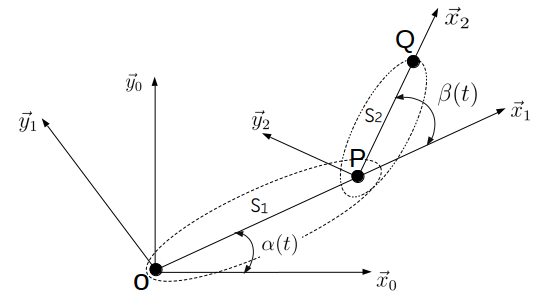
\includegraphics[scale=0.5]{graph_exam.png}

\end{figure}

\begin{itemize}
\item[1)] Exprimer les vecteurs de rotations instantannées $\vec{\Omega}(b_1/b_0)$, $\vec{\Omega}(b_2/b_1)$ et $\vec{\Omega}(b_2/b_0)$
\item[2)] Calculer les vitesses et accélérations des points P et Q par rapport à $\mathcal{R}_0$ (on pourra utiliser les formules démontrées plus haut).
\item[3)] Calculer la vitesse et l'accéleration du point Q par rapport à $\mathcal{R}_1$.
\vspace{2mm}
\end{itemize}
\vspace{5mm}

\pagebreak

$$ \mathcal{D} = \left\lbrace \ \underbrace{\bepar{\eta_1,\eta_2,\, ...\,, \eta_n}}_{X_i}, \ \underbrace{\beta_i}_{y_i}\ \right\rbrace $$
	


\end{document}